
\chapter{An\'alise de Dispers\~ao e Atenua\c{c}\~ao}\label{sec.app_faraday}
Para o caso citado na subse\c{c}\~ao \ref{sec.faraday}, calculamos a velocidade de fase e atenua\c{c}\~ao de ondas mec\^anicas e eletromagn\'eticas considerando as componentes $u_1$, $u_2$ e $H_3$, escolhendo a dire\c{c}\~ao horizontal de propaga\c{c}\~ao dessas ondas. O gr\'afico \ref{fig.disp_fa_45}  mostra a propaga\c{c}\~ao na dire\c{c}\~ao $45^\circ$ no plano $xy$ e foi confeccionado usando a ferramenta \textit{root} para extrair as ra\'izes de um polin\^omio de grau 6. Observamos o mesmo comportamento da an\'alise feita na subse\c{c}\~ao \ref{sec.faraday}, com a diferen\c{c}a do problema num\'erico gerado pela ferramenta \textit{root}. 

\begin{figure}
\centering
\subfloat{\includegraphics[scale=.425]{app_v_u}}
\subfloat{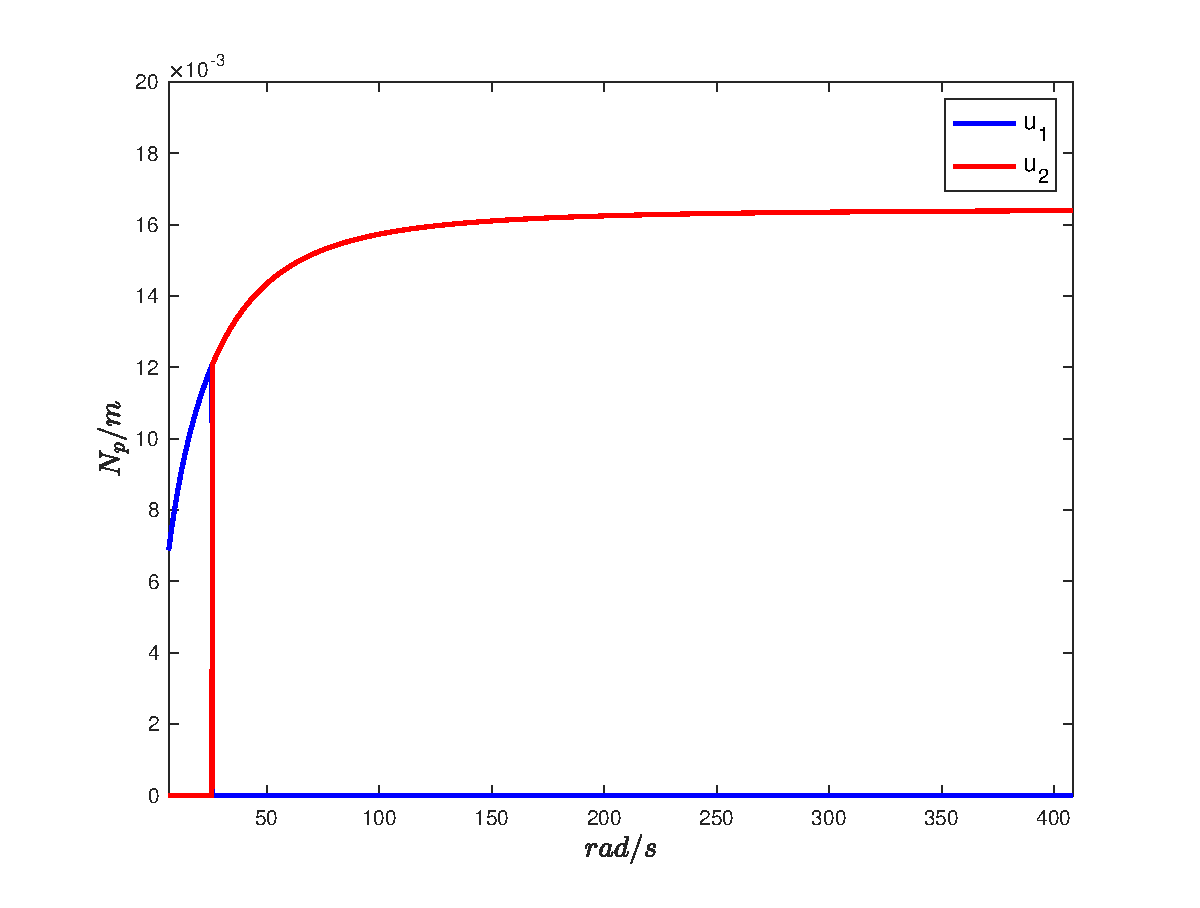
\includegraphics[scale=.425]{app_at_u}}\\
%\subfloat{\includegraphics[scale=.57]{phase_veloc_faraday_3}}
%\subfloat{\includegraphics[scale=.57]{attenuation_faraday_3}}\\
\subfloat{\includegraphics[scale=.425]{app_v_h}}
\subfloat{\includegraphics[scale=.425]{app_at_h}}
\caption{\textit{Velocidade de fase e atenua\c{c}\~ao de duas ondas el\'asticas e de uma onda eletromagn\'etica, que se propagam na dire\c{c}\~ao de $45^\circ$ no plano $xy$, e em fun\c{c}\~ao da frequ\^encia angular e de um campo magn\'etico externo. Caso Faraday.}}
\label{fig.disp_fa_45}
\end{figure}


\chapter{Modelo com Duas Fontes: S\'ismica e Eletromagn\'etica}
Normalmente, em levantamentos s\'ismicos s\~ao utilizadas somente fontes de ondas mec\^anicas, mas \'e poss\'ivel obtermos alguns resultados te\'oricos utilizando dois tipos de fontes simultaneamente. A seguir verificamos a inclus\~ao de uma fonte eletromagn\'etica junto com a fonte s\'ismica para o modelo de propaga\c{c}\~ao de ondas em meio 1D, homog\^eneo e com acoplamento total entre campos mec\^anicos e eletromagn\'eticos.

Incluindo uma fonte eletromagn\'etica $f(z,t)$ no sistema TAL, temos
\begin{align}
-\omega^2\rho\,u&=\frac{\partial}{\partial\,z}\left[(\lambda+2\,G)\frac{\partial\,u}{\partial\,z}-\mu h^0h\right]+F(z,\omega)\\\nonumber\\\
-i\,\omega\,h&=\frac{\partial}{\partial\,z}\left(V_H\frac{\partial\,h}{\partial\,z}-h^0\frac{\partial\,u}{\partial\,t}\right)-V_H f(z,t).
\end{align}
As solu\c{c}\~oes para esse novo sistema com duas fontes s\~ao dadas por 
\begin{align*}
u(k,\omega)&=u_1(k,\omega)+g_2(k,\omega)\,h_1(k,\omega)\\
h(k,\omega)&=g_1(k,\omega)\,u_1(k,\omega)+h_1(k,\omega),
\end{align*}
onde,
\begin{align*}
g_2(k,\omega)&=\frac{-i\,k\,\mu_0h^0}{(\lambda+2\,G)k^2-\omega^2\rho}\\\\
u_1(k,\omega)&=\frac{F}{(\lambda+2\,G)\,k^2-\omega^2\rho+i\,k\,\mu_0h^0g_1}\\\\
h_1(k,\omega)&=\frac{-V_Hf}{V_Hk^2-\omega^2\rho+k\,\omega\,h^0g_2}.
\end{align*}
Finalmente, se o acoplamento das ondas \'e parcial, temos
\begin{align*}
u_p(k,\omega)&=\frac{F}{(\lambda+2\,G)\,k^2-\omega^2\rho}\\
h_p(k,\omega)&=g_1(k,\omega)\,u_p(k,\omega)-\frac{V_Hf}{V_Hk^2-\omega^2\rho} .
\end{align*}
Observe que, para sistemas parcialmente acoplados, a solu\c{c}\~ao para ondas mec\^anicas permanece sem influ\^encia de for\c{c}as eletromagn\'eticas mesmo com a inclus\~ao de uma fonte eletromagn\'etica junto com a fonte s\'ismica. 

\begin{figure}
\centering
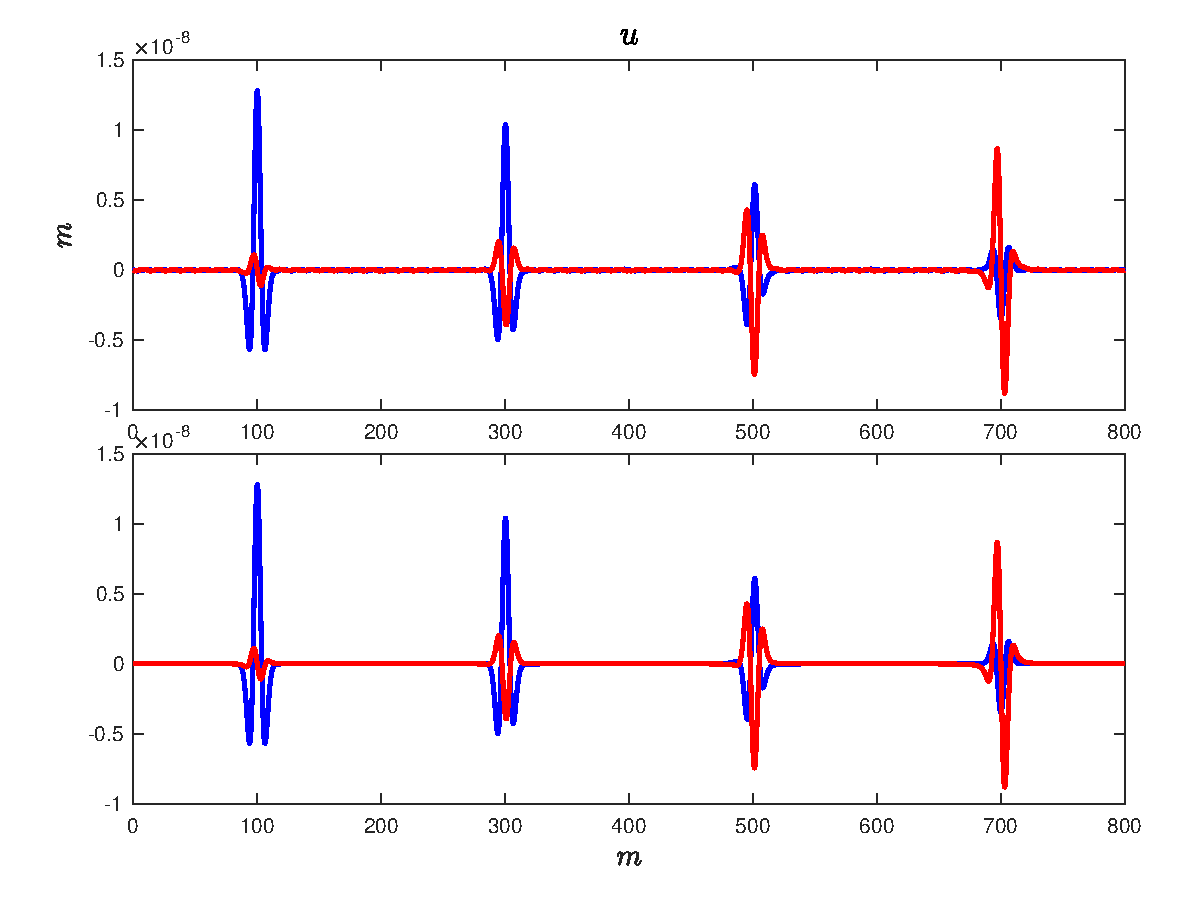
\includegraphics[scale=.73]{u_homo_Ff}
\caption{\textit{Considerando duas fontes, temos a amplitude de onda mec\^anica para sistema totalmente acoplado em cima e parcialmente acoplado embaixo.}}
\end{figure}

\begin{figure}
\centering
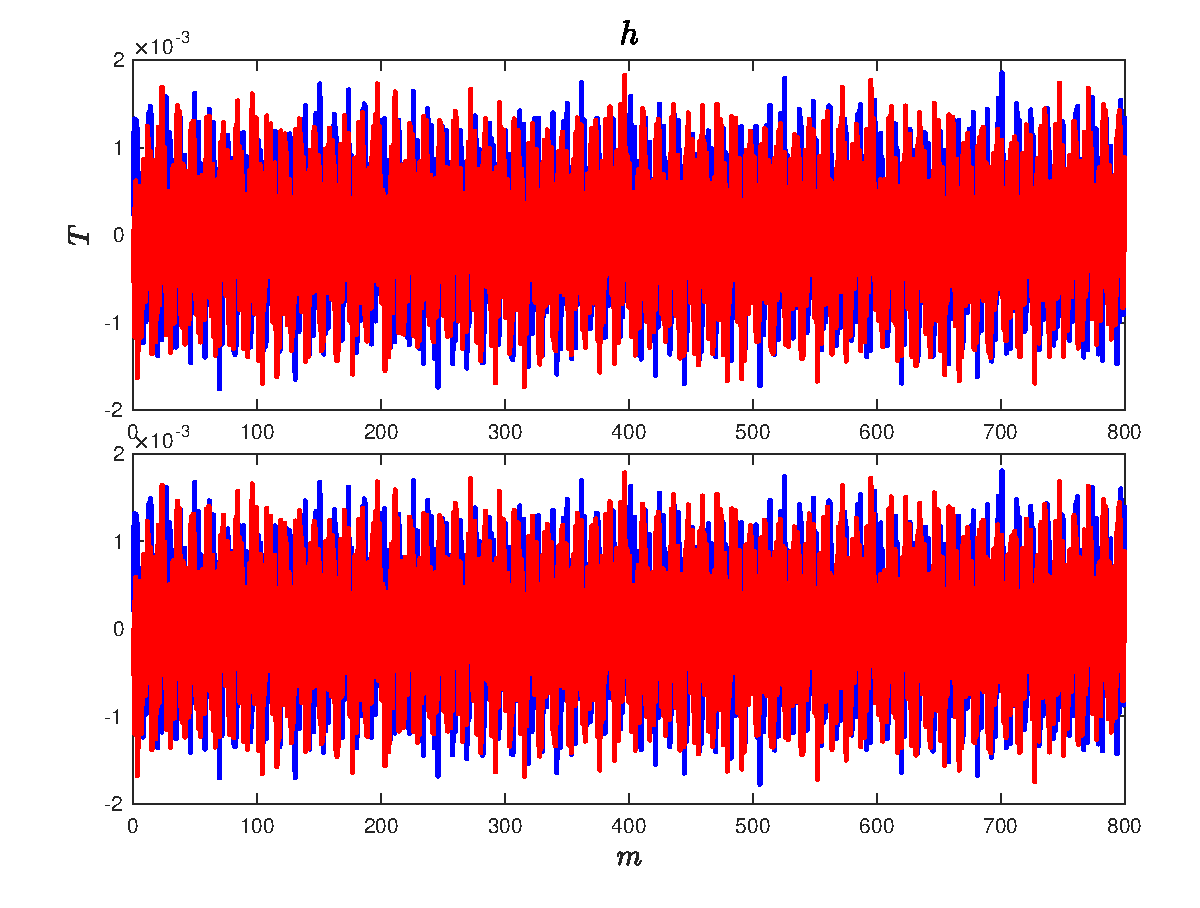
\includegraphics[scale=.73]{h_homo_Ff}
\caption{\textit{Considerando duas fontes, temos a amplitude da varia\c{c}\~ao magn\'etica para sistema totalmente acoplado em cima e parcialmente acoplado embaixo.}}
\end{figure}

TO CITE THE GRAPHICS in THE BODY TEXT\\
TO BUILD ANOTHER GRAPHICS CONSIDERING THE MAGNETIC VISCOSITY AT ELECTROMAGNETIC SOURCE.\\
THE ELECTROMAGNETIC SOURCE PRODUCE A LOT'S OF NOISES IN THE GRAPHICS (SPECIALLY IF WE INCLUDE VH) AND WE WILL PUSH THAT MODEL TO APPENDIX.



